\section{Pubblicità}\label{pubblicita}

Su TicketOne le pubblicità possono sembrare assenti, mentre,  in realtà, sono inserite in maniera molto intelligente all'interno del contenuto proposto.
Questo viene fatto attraverso il \textit{blending}, ovvero posizionare i banner pubblicitari all'interno del contenuto invece che mantenerli nelle sezioni più utilizzate.
\par Le pubblicità che vengono proposte, oltre ad essere presentate insieme agli eventi, sono inerenti ad attività, luoghi, altri eventi o applicazioni simili che possono interessare l'utente.

\subsection{Posizionamento e contenuti}
	La maggior parte delle inserzioni pubblicitarie proposte sono contenute all'interno dell'homepage (allegata in \textit{pdf}).
	Queste sono posizionate in due sezioni, (la colonna di sinistra e il contenitore centrale), che iniziano dopo il carosello degli eventi principali.
	\par Come mostrato in Fig.~\ref{fig:pub1} e Fig.~\ref{fig:pub2}, la colonna di sinistra è formata da annunci e offerte interne a TicketOne, classifiche di eventi e pubblicità che portano a siti esterni che sono strettamente correlati a quello che offre il sito in analisi.
	In particolare la pubblicità relativa agli eventi calcistici in Fig.~\ref{fig:pub2}.
	\par Nella sezione centrale della pagina, le pubblicità vengono alternate alle righe che suddividono gli eventi per categoria.
	Queste sono denominate come ``\textit{In evidenza}'' e, come per la colonna di sinistra, contengono pubblicità relative a TicketOne oltre a luoghi o eventi esterni al sito.
	Un paio di esempi sono le inserzioni relative al \textit{Teatro alla Scala}, in Fig.~\ref{fig:pub1}, e alle modalita in cui spendere il buono ``\textit{Carta del docente}'' in Fig.~\ref{fig:pub2}.
	\par Una nota positiva è l'assenza di pubblicità con animazioni che possono distrarre l'utente e, se eccessive, potrebbero addirittura farlo ``scappare''.
	Questo tipo di pubblicità, oltre ad avere un impatto negativo sull'esperienza degli utenti, possono anche aumetare il tempo di caricamento delle pagine.

\begin{figure}
	\makebox[\textwidth][c]{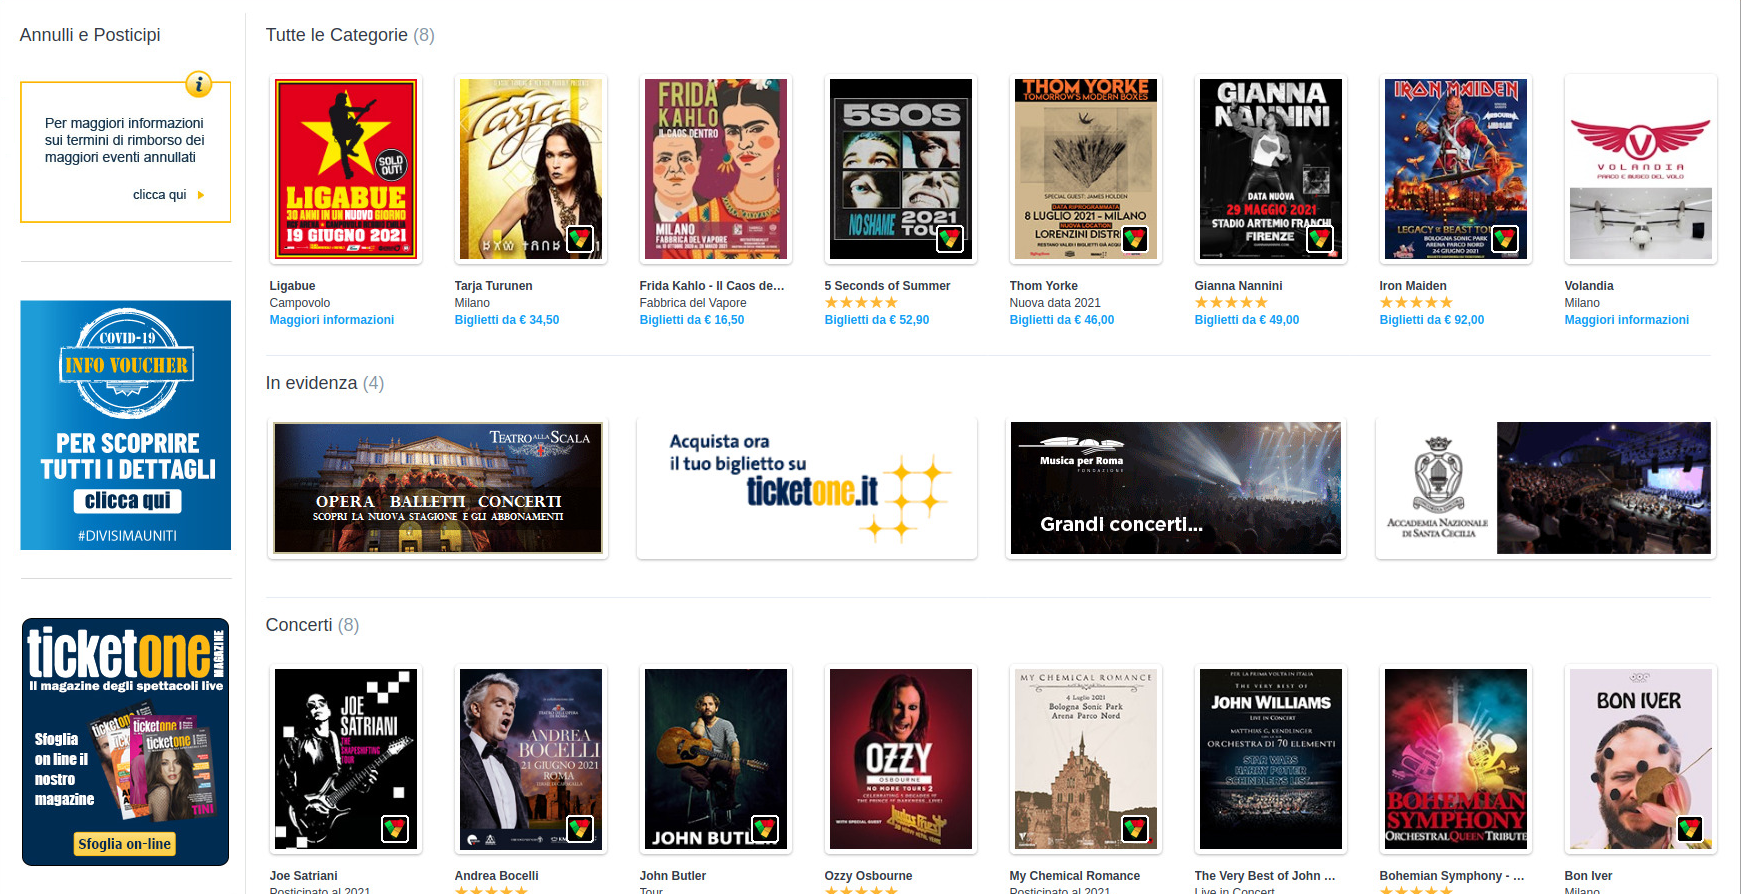
\includegraphics[width=1.3\textwidth]{img/pubblicita_1.png}}%
	\caption{Primo esempio di pubblicità in TicketOne}
	\label{fig:pub1}
\end{figure}

\begin{figure}
	\makebox[\textwidth][c]{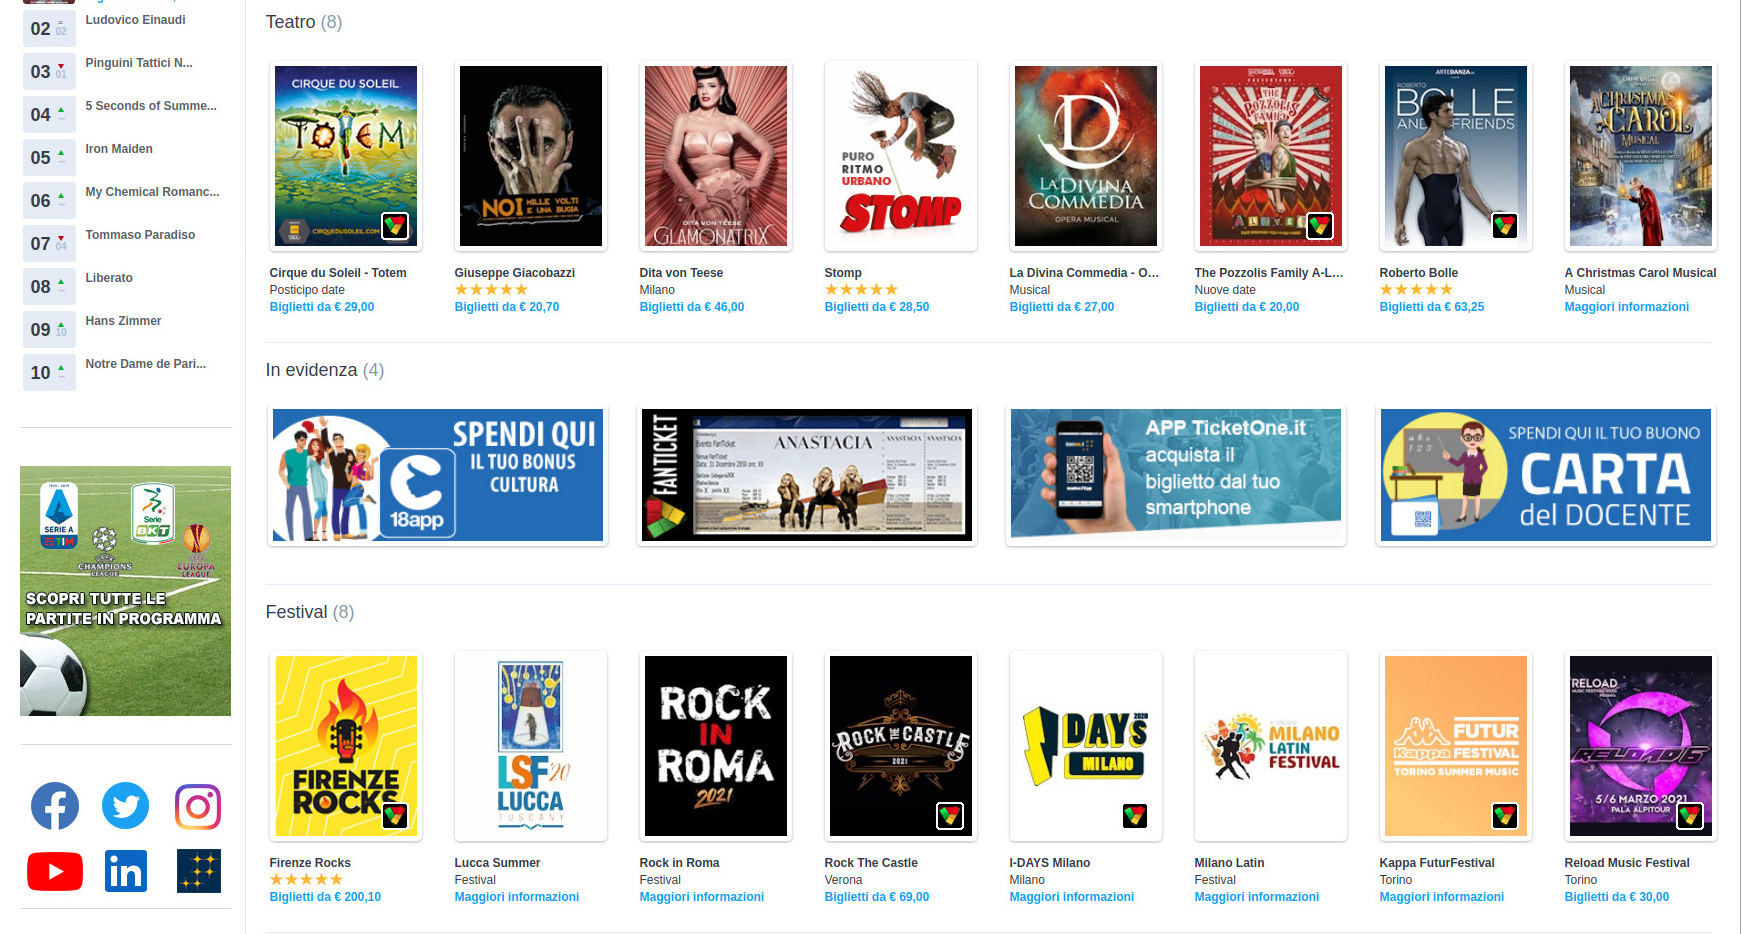
\includegraphics[width=1.3\textwidth]{img/pubblicita_2.png}}%
	\caption{Secondo esempio di pubblicità in TicketOne}
	\label{fig:pub2}
\end{figure}